\documentclass[landscape,a0paper,fontscale=0.292]{baposter}

\usepackage[vlined]{algorithm2e}
\usepackage{times}
\usepackage{calc}
\usepackage{url}
\usepackage{graphicx}
\usepackage{amsmath}
\usepackage{amssymb}
\usepackage{relsize}
\usepackage{multirow}
\usepackage{booktabs}

\usepackage{makecell}

\usepackage{graphicx}
\usepackage{multicol}
\usepackage[T1]{fontenc}
\usepackage{ae}

\graphicspath{{images/}}

 %%%%%%%%%%%%%%%%%%%%%%%%%%%%%%%%%%%%%%%%%%%%%%%%%%%%%%%%%%%%%%%%%%%%%%%%%%%%%%%%
 %%%% Some math symbols used in the text
 %%%%%%%%%%%%%%%%%%%%%%%%%%%%%%%%%%%%%%%%%%%%%%%%%%%%%%%%%%%%%%%%%%%%%%%%%%%%%%%%
 % Format
 \newcommand{\RotUP}[1]{\begin{sideways}#1\end{sideways}}


 %%%%%%%%%%%%%%%%%%%%%%%%%%%%%%%%%%%%%%%%%%%%%%%%%%%%%%%%%%%%%%%%%%%%%%%%%%%%%%%%
 % Multicol Settings
 %%%%%%%%%%%%%%%%%%%%%%%%%%%%%%%%%%%%%%%%%%%%%%%%%%%%%%%%%%%%%%%%%%%%%%%%%%%%%%%%
 \setlength{\columnsep}{0.7em}
 \setlength{\columnseprule}{0mm}


 %%%%%%%%%%%%%%%%%%%%%%%%%%%%%%%%%%%%%%%%%%%%%%%%%%%%%%%%%%%%%%%%%%%%%%%%%%%%%%%%
 % Save space in lists. Use this after the opening of the list
 %%%%%%%%%%%%%%%%%%%%%%%%%%%%%%%%%%%%%%%%%%%%%%%%%%%%%%%%%%%%%%%%%%%%%%%%%%%%%%%%
 \newcommand{\compresslist}{%
 \setlength{\itemsep}{1pt}%
 \setlength{\parskip}{0pt}%
 \setlength{\parsep}{0pt}%
 }


 %%%%%%%%%%%%%%%%%%%%%%%%%%%%%%%%%%%%%%%%%%%%%%%%%%%%%%%%%%%%%%%%%%%%%%%%%%%%%%
 % Formating
 \newcommand{\Matrix}[1]{\begin{bmatrix} #1 \end{bmatrix}}
 \newcommand{\Vector}[1]{\begin{pmatrix} #1 \end{pmatrix}}

 \newcommand*{\norm}[1]{\mathopen\| #1 \mathclose\|}% use instead of $\|x\|$
 \newcommand*{\abs}[1]{\mathopen| #1 \mathclose|}% use instead of $\|x\|$
 \newcommand*{\normLR}[1]{\left\| #1 \right\|}% use instead of $\|x\|$

 \newcommand*{\SET}[1]  {\ensuremath{\mathcal{#1}}}
 \newcommand*{\FUN}[1]  {\ensuremath{\mathcal{#1}}}
 \newcommand*{\MAT}[1]  {\ensuremath{\boldsymbol{#1}}}
 \newcommand*{\VEC}[1]  {\ensuremath{\boldsymbol{#1}}}
 \newcommand*{\CONST}[1]{\ensuremath{\mathit{#1}}}

 \DeclareMathOperator*{\argmax}{arg\,max}
 \DeclareMathOperator*{\diag}{diag}
 \DeclareMathOperator*{\argmin}{arg\,min}
 \DeclareMathOperator*{\vectorize}{vec}
 \DeclareMathOperator*{\reshape}{reshape}

 %-----------------------------------------------------------------------------
 % Differentiation
 \newcommand*{\Nabla}[1]{\nabla_{\!#1}}

 \renewcommand*{\d}{\mathrm{d}}
 \newcommand*{\dd}{\partial}

 \newcommand*{\At}[2]{\ensuremath{\left.#1\right|_{#2}}}
 \newcommand*{\AtZero}[1]{\At{#1}{\pp=\VEC 0}}

 \newcommand*{\diffp}[2]{\ensuremath{\frac{\dd #1}{\dd #2}}}
 \newcommand*{\diffpp}[3]{\ensuremath{\frac{\dd^2 #1}{\dd #2 \dd #3}}}
 \newcommand*{\diffppp}[4]{\ensuremath{\frac{\dd^3 #1}{\dd #2 \dd #3 \dd #4}}}
 \newcommand*{\difff}[2]{\ensuremath{\frac{\d #1}{\d #2}}}
 \newcommand*{\diffff}[3]{\ensuremath{\frac{\d^2 #1}{\d #2 \d #3}}}
 \newcommand*{\difffp}[3]{\ensuremath{\frac{\dd\d #1}{\d #2 \dd #3}}}
 \newcommand*{\difffpp}[4]{\ensuremath{\frac{\dd^2\d #1}{\d #2 \dd #3 \dd #4}}}

 \newcommand*{\diffpAtZero}[2]{\ensuremath{\AtZero{\diffp{#1}{#2}}}}
 \newcommand*{\diffppAtZero}[3]{\ensuremath{\AtZero{\diffpp{#1}{#2}{#3}}}}
 \newcommand*{\difffAt}[3]{\ensuremath{\At{\difff{#1}{#2}}{#3}}}
 \newcommand*{\difffAtZero}[2]{\ensuremath{\AtZero{\difff{#1}{#2}}}}
 \newcommand*{\difffpAtZero}[3]{\ensuremath{\AtZero{\difffp{#1}{#2}{#3}}}}
 \newcommand*{\difffppAtZero}[4]{\ensuremath{\AtZero{\difffpp{#1}{#2}{#3}{#4}}}}

 %-----------------------------------------------------------------------------
 % Defined
 % How should the defined operator look like (:= or ^= ==)
 % (I want back my :=, it is so much better than ^= because (1) it has a
 % direction and (2) everyone here uses it.)
 %
 % Use :=
 %\newcommand*{\defined}{\ensuremath{\mathrel{\mathop{:}}=}}
 %\newcommand*{\definedRight}{\ensuremath{=\mathrel{\mathop{:}}}}
 % Use ^=
 \newcommand*{\defined}{\ensuremath{\triangleq}}
 \newcommand*{\definedRight}{\ensuremath{\triangleq}}
 % Use = with three bars
 %\newcommand*{\defined}{\ensuremath{?}}
 %\newcommand*{\definedRight}{\ensuremath{?}}

 %%%%%%%%%%%%%%%%%%%%%%%%%%%%%%%%%%%%%%%%%%%%%%%%%%%%%%%%%%%%%%%%%%%%%%%%%%%%%%
 % Symbols used in the paper

 %-----------------------------------------------------------------------------
 % The Methods
 \newcommand*{\ICIA}{\emph{ICIA}}
 \newcommand*{\CoDe}{\emph{CoDe}}
 \newcommand*{\LinCoDe}{\emph{LinCoDe}}
 \newcommand*{\CoNe}{\emph{CoNe}}
 \newcommand*{\CoLiNe}{\emph{CoLiNe}}
 \newcommand*{\LinCoLiNe}{\emph{LinCoLiNe}}

 % inter eye distance
 \newcommand*{\ied}{IED}

 %-----------------------------------------------------------------------------
 % Koerper
 %%\newcommand*{\RR}{\mathbb{R}}
 %\newcommand*{\RR}{{I\hspace{-3.5pt}R}}
 %\newcommand*{\RR}{{\mathrm{I\hspace{-2.7pt}R}}}

 \font\dsfnt=dsrom12

 \DeclareSymbolFont{nark}{U}{dsrom}{m}{n}
 \DeclareMathSymbol{\NN}{\dsfnt}{nark}{`N}
 \DeclareMathSymbol{\RR}{\dsfnt}{nark}{`R}
 \DeclareMathSymbol{\ZZ}{\dsfnt}{nark}{`Z}

 %-----------------------------------------------------------------------------
 % Domains
 \newcommand*{\D}{\mathcal{D}}
 \newcommand*{\I}{\mathcal{I}}

 %-----------------------------------------------------------------------------
 % Texture coordinates
 \newcommand*{\rr}{\VEC{r}}

 %-----------------------------------------------------------------------------
 % Parameters
 \newcommand*{\pt}{\VEC{\tau}}
 \newcommand*{\pr}{\VEC{\rho}}
 \newcommand*{\pp}{\VEC{p}}
 \newcommand*{\qq}{\VEC{q}}
 \newcommand*{\xx}{\VEC{x}}
 \newcommand*{\deltaq}{\Delta \qq}
 \newcommand*{\deltap}{\Delta \pp}
 \newcommand*{\zz}{\VEC{z}}
 \newcommand*{\pa}{\VEC{\alpha}}
 \newcommand*{\qa}{\VEC{\alpha}}
 \newcommand*{\pb}{\VEC{\beta}}

 %-----------------------------------------------------------------------------
 % Optimal appearance parameters
 \newcommand*{\pbh}[1]{\ensuremath{\hat{\pb}({#1})}}

 %-----------------------------------------------------------------------------
 % Warp basis
 \newcommand*{\M}[1]{\ensuremath{M({#1})}}
 \newcommand*{\LL}[1]{\ensuremath{L({#1})}}

 %-----------------------------------------------------------------------------
 % Matrices of the texture model
 \newcommand*{\AM}[1]{\ensuremath{\Lambda(#1)}}               % Lambda(beta)
 \newcommand*{\AMr}[2]{\ensuremath{\Lambda(#1; #2)}}        % Lambda(r, beta)

 \newcommand*{\As}{A}         % Continuous Basis symbol
 \newcommand*{\afs}{a}        % Continuous mean symbol
 \newcommand*{\A}[1]{\As(#1)}         % Continuous Basis
 \newcommand*{\af}[1]{\afs(#1)}        % Continuous mean


 %-----------------------------------------------------------------------------
 % Matrices of the shape model
 \newcommand*{\MU}{\VEC{\mu}}
 \newcommand*{\MM}{\MAT{M}}

 %-----------------------------------------------------------------------------
 %% The project out matrix and operator
 \newcommand*{\INT}{\MAT{P}}
 \newcommand*{\INTf}{P}

 %-----------------------------------------------------------------------------
 % The identity matrix
 \newcommand*{\EYEtwo}{\Matrix{1 & 0\\0&1}}
 \newcommand*{\EYE}{\MAT E}
 \newcommand*{\EYEf}{E}

 % Wether to use subscripts or brackets for some function arguments
 % can be decided by commenting out the corresponding functions underneath
 %-----------------------------------------------------------------------------
 % Mapping
 \newcommand*{\Cs}[1]{\ensuremath{C^{#1}}} % C symbol
 \newcommand*{\C}[2]{\ensuremath{C^{#1}(#2)}} % Use C with brackets

 %-----------------------------------------------------------------------------
 % Objective function
 \newcommand*{\Fs}{\ensuremath{F}}              % F symbol
 \newcommand*{\F}[1]{\ensuremath{\Fs(#1)}}       % Use F with brackets    F(q)

 %-----------------------------------------------------------------------------
 % Approximated objective functions
 \newcommand*{\FFs}{\tilde{F}}                     % ~F symbol
 \newcommand*{\FF}[1]{\ensuremath{\FFs(#1)}}       % Use ~F with brackets    F(q)

 %-----------------------------------------------------------------------------
 % residual function
 \newcommand*{\es}{\ensuremath{f}}              % R symbol

 \newcommand*{\e}[1]{\ensuremath{\es(#1)}}         % R(q)
 \newcommand*{\er}[2]{\ensuremath{\es(#1; #2)}}    % R(r; q)

 %-----------------------------------------------------------------------------
 % Approximated residual functions
 \newcommand*{\ees}{\tilde{f}}                       % ~R symbol
 \newcommand*{\ee}[1]{\ensuremath{\ees(#1)}}       % ~R(q)
 \newcommand*{\eer}[2]{\ensuremath{\ees(#2; #1)}}  % ~R(r; q)

 %-----------------------------------------------------------------------------
 % Warps
 \newcommand*{\Vs}{\ensuremath{V}}
 \newcommand*{\VLins}{\ensuremath{\Vs^{\text{Ortho}}}}
 \newcommand{\VModels}{\ensuremath{\Vs^{\text{Model}}}}
 \newcommand*{\Ws}{\ensuremath{W}}

 \newcommand{\V}[1]{\ensuremath{\Vs(#1)}}
 \newcommand{\VModel}[1]{\ensuremath{\VModels(#1)}}
 \newcommand{\Vr}[2]{\ensuremath{\Vs(#1; #2)}}
 \newcommand{\VInvr}[2]{\ensuremath{\Vs^{-1}(#1; #2)}}
 \newcommand{\VrLin}[2]{\ensuremath{\VLins(#1; #2)}}
 \newcommand{\W}[1]{\ensuremath{\Ws(#1)}}
 \newcommand{\Winv}[1]{\ensuremath{\Ws^{-1}(#1)}}
 \newcommand{\Wr}[2]{\ensuremath{\Ws(#1; #2)}}


%%%%%%%%%%%%%%%%%%%%%%%%%%%%%%%%%%%%%%%%%%%%%%%%%%%%%%%%%%%%%%%%%%%%%%%%%%%%%
%% Begin of Document
%%%%%%%%%%%%%%%%%%%%%%%%%%%%%%%%%%%%%%%%%%%%%%%%%%%%%%%%%%%%%%%%%%%%%%%%%%%%%
\begin{document}
%%%%%%%%%%%%%%%%%%%%%%%%%%%%%%%%%%%%%%%%%%%%%%%%%%%%%%%%%%%%%%%%%%%%%%%%%%%%%
%% Here starts the poster
%%---------------------------------------------------------------------------
%% Format it to your taste with the options
%%%%%%%%%%%%%%%%%%%%%%%%%%%%%%%%%%%%%%%%%%%%%%%%%%%%%%%%%%%%%%%%%%%%%%%%%%%%%
\begin{poster}{
		% Show grid to help with alignment
		grid=false,
		% Column spacing
		colspacing=0.7em,
		% Color style
		headerColorOne=red!20!white!90!black,
		borderColor=red!30!white!90!black,
		% Format of textbox
		textborder=faded,
		% Format of text header
		headerborder=open,
		headershape=roundedright,
		headershade=plain,
		background=none,
		bgColorOne=red!10!white,
		headerheight=0.17\textheight}
	% Eye Catcher
	% Title
	{\sc\huge
		\textbf{Running Large and Dynamic Climate Ensembles in the Cloud}
		
\includegraphics[width=0.12\linewidth]{images/logo_ephyslab}}
	% Authors
	{
		\textbf{Running Large and Dynamic Climate Ensembles in the Cloud}
	}
	{\vskip0.5cm Diego Montes$^{1}$, Juan A. A\~nel$^{1}$, Javier Rodeiro$^{2}$\\~\\
		{\texttt{email: kabute@uvigo.es}}
		\small{\texttt{\begin{center}$^{1}$ University of Vigo, EPhysLab, Ourense, Spain, $^{2}$ University
			of Vigo, School of Informatics Engineering, Ourense, Spain  \end{center}}}}

	% University logo
	% {
	%  \begin{tabular}{r}
	%\includegraphics[height=0.12\textheight]{logo}\\
	%\raisebox{0em}[0em][0em]{\includegraphics[height=0.03\textheight]{msrlogo}}
	%  \end{tabular}
	% }

	%%%%%%%%%%%%%%%%%%%%%%%%%%%%%%%%%%%%%%%%%%%%%%%%%%%%%%%%%%%%%%%%%%%%%%%%%%%%%%
	%%% Now define the boxes that make up the poster
	%%%---------------------------------------------------------------------------
	%%% Each box has a name and can be placed absolutely or relatively.
	%%% The only inconvenience is that you can only specify a relative position
	%%% towards an already declared box. So if you have a box attached to the
	%%% bottom, one to the top and a third one which should be inbetween, you
	%%% have to specify the top and bottom boxes before you specify the middle
	%% box.
	%%%%%%%%%%%%%%%%%%%%%%%%%%%%%%%%%%%%%%%%%%%%%%%%%%%%%%%%%%%%%%%%%%%%%%%%%%%%%%


	%%%%%%%%%%%%%%%%%%%%%%%%%%%%%%%%%%%%%%%%%%%%%%%%%%%%%%%%%%%%%%%%%%%%%%%%%%%%%%
	\headerbox{\textbf{\textcolor{white}{Problem Background}}}{name=background,column=0,span=2}{
		%%%%%%%%%%%%%%%%%%%%%%%%%%%%%%%%%%%%%%%%%%%%%%%%%%%%%%%%%%%%%%%%%%%%%%%%%%%%%%
		%\vspace{-0.5em}
		\begin{itemize}
			\item Climate and meteorological oriented software and simulations usage in Cloud Systems is growing and has proven to be a feasible and solid solution for these kind of scientific applications.
			\item This approach allows scientists to reduce toil and burden (e.g. infrastructure setup and troubleshooting).
			\item Our most recent work has the focus on providing an out-of-the-box solution for WRF that works on diverse environments, specially public clouds.
		\end{itemize}
	}

	%%%%%%%%%%%%%%%%%%%%%%%%%%%%%%%%%%%%%%%%%%%%%%%%%%%%%%%%%%%%%%%%%%%%%%%%%%%%%%
	\headerbox{\textbf{\textcolor{white}{Goals}}}{name=goals,column=0,row=0,span=2,below=background}{
		%%%%%%%%%%%%%%%%%%%%%%%%%%%%%%%%%%%%%%%%%%%%%%%%%%%%%%%%%%%%%%%%%%%%%%%%%%%%%%
		\begin{itemize}
			\item Provide an idempotent out-of-the-box solution that could be reused in a wide range of environments to run Climate simulations.
			\item Create a simplified workflow so, scientists using this solution can focus their efforts on doing science rather than setting up hardware or software that adds little value to their research.
		\end{itemize}

	}
	%%%%%%%%%%%%%%%%%%%%%%%%%%%%%%%%%%%%%%%%%%%%%%%%%%%%%%%%%%%%%%%%%%%%%%%%%%%%%%
	\headerbox{\textbf{\textcolor{white}{Proposed Solution}}}{name=solution,column=0,row=0,span=2,below=goals}{
		%%%%%%%%%%%%%%%%%%%%%%%%%%%%%%%%%%%%%%%%%%%%%%%%%%%%%%%%%%%%%%%%%%%%%%%%%%%%%%
		\begin{center}
			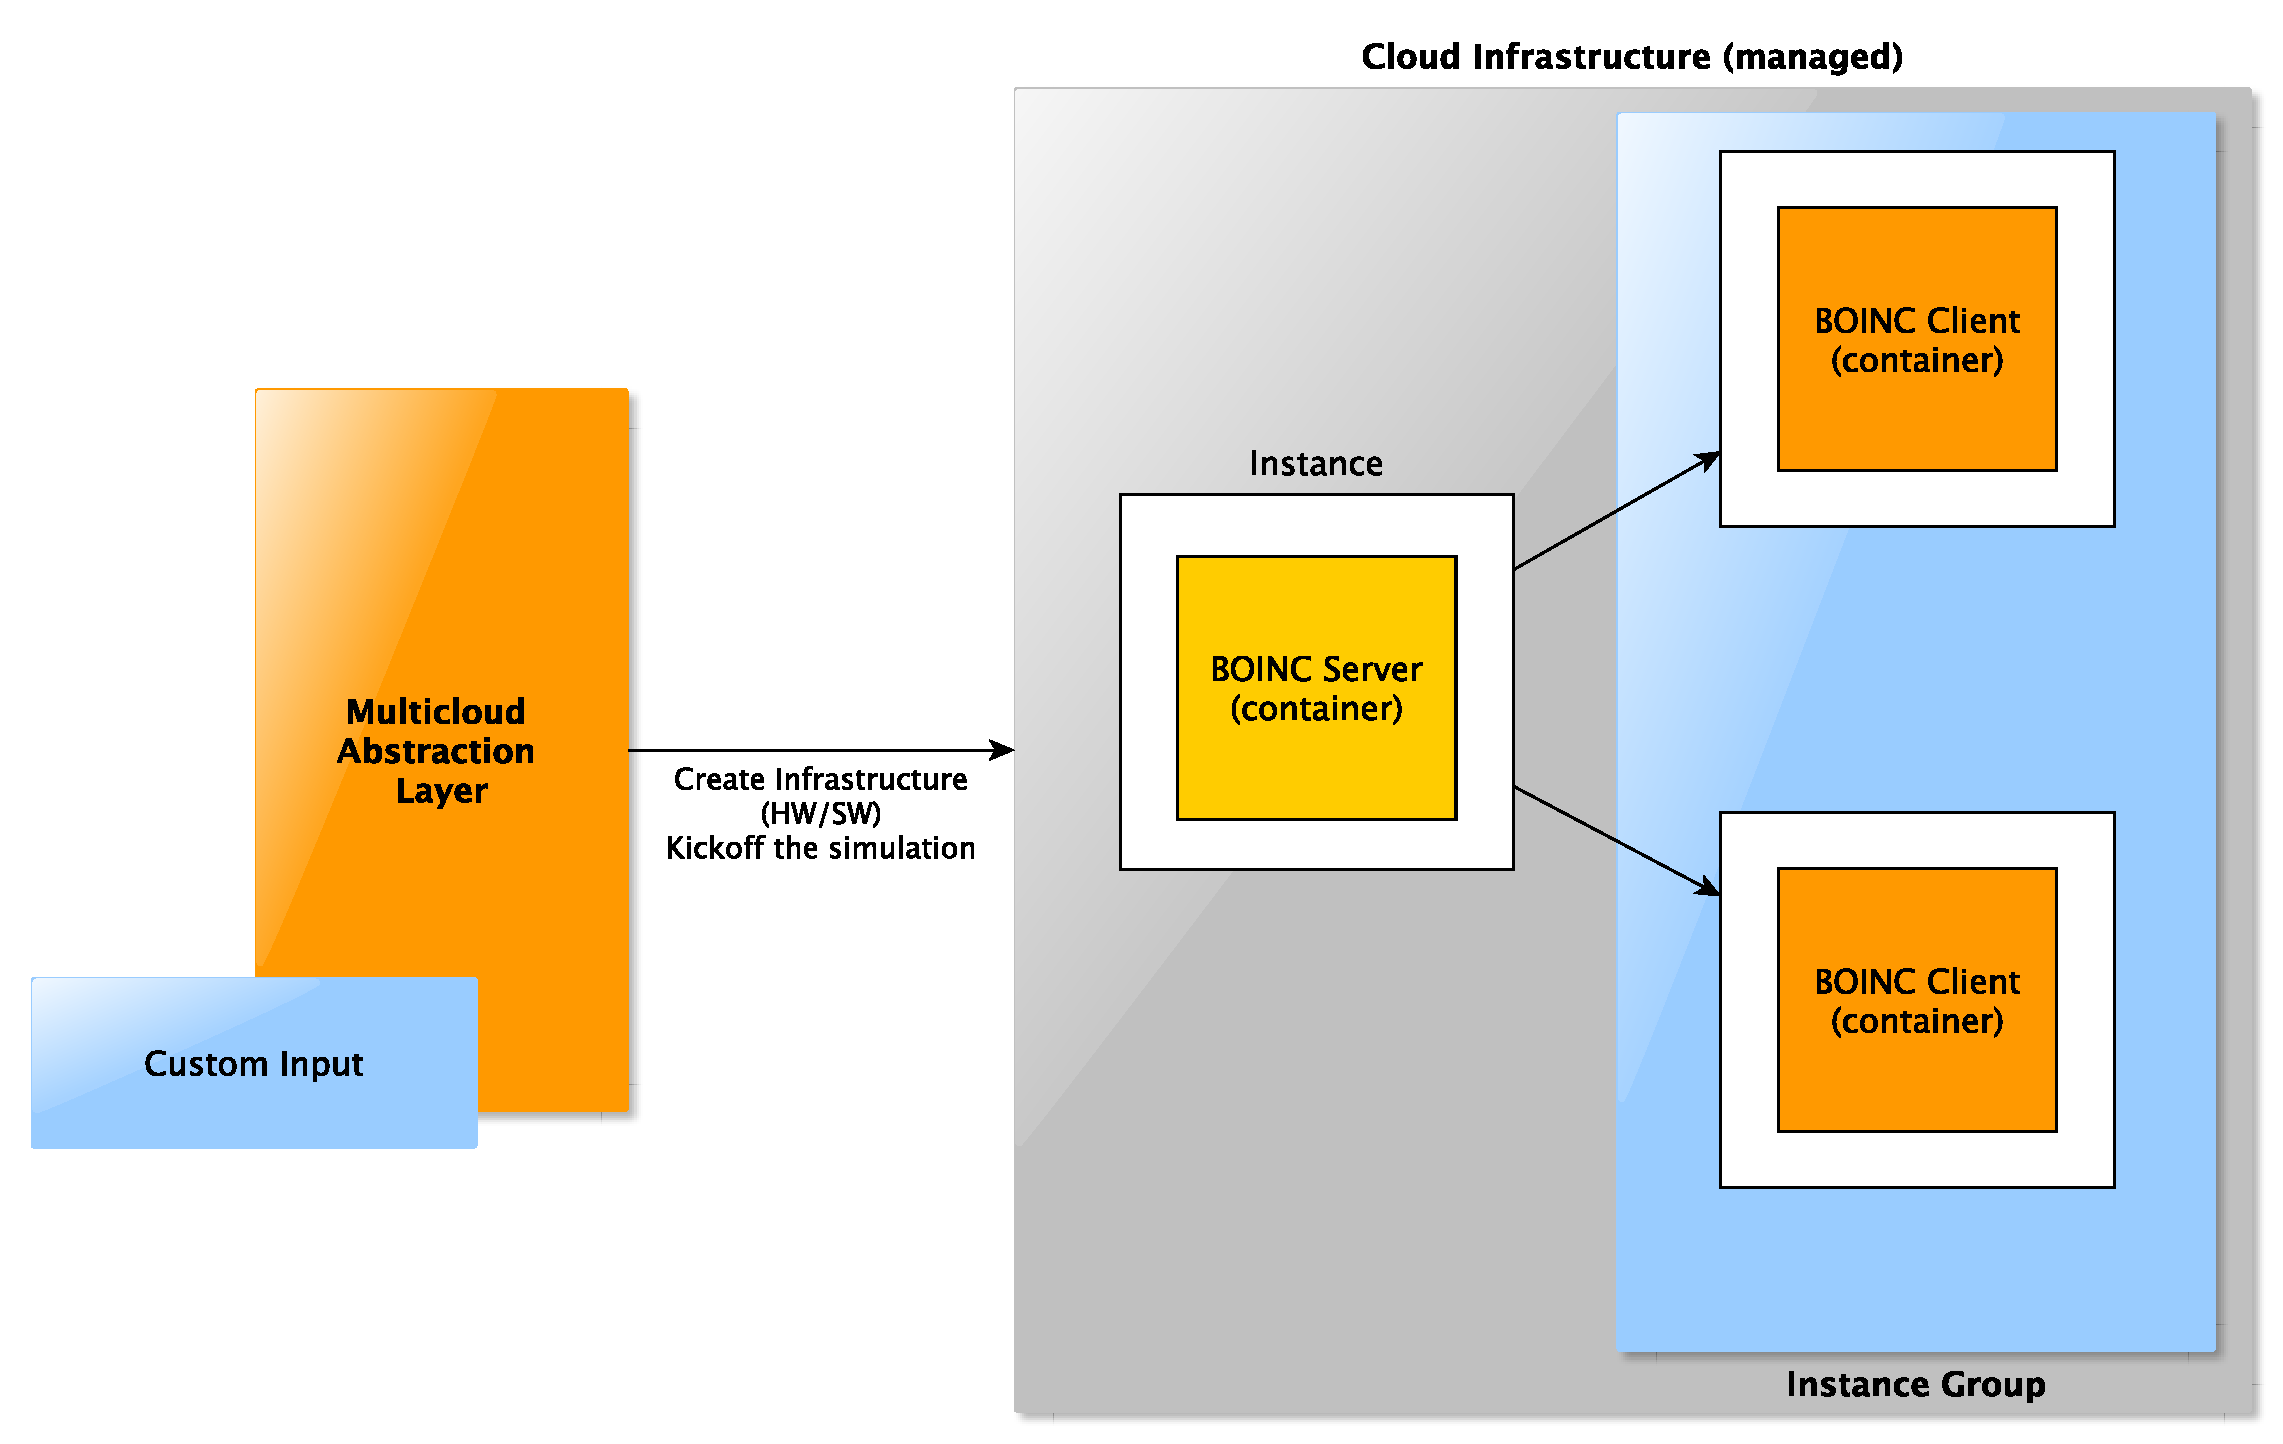
\includegraphics[height=18.25em]{images/architecture}\\
			{\footnotesize \textbf{Figure 1.}Proposed Solution Highe Level Architecture.\\~\\}
				\end{center}
				Our proposal is a highly abstracted multi-cloud solution with the following components:
				\begin{itemize}
					\item A \textbf{Multicloud abstraction layer} that uses in-house developed software that generates (from given custom inputs) the needed outputs (e.g. configured docker images and templates) so they can be consumed in an infrastructure as code solution and create the needed artifacts (both software and target infrastructure) and run the simulation.
					\item \textbf{Fully automated infrastructure} that runs WRF inside BOINC (by using the usual server/client architecture) with the inputs that the management layer created.
				\end{itemize}
			}


			%%%%%%%%%%%%%%%%%%%%%%%%%%%%%%%%%%%%%%%%%%%%%%%%%%%%%%%%%%%%%%%%%%%%%%%%%%%%%%
			\headerbox{\textbf{\textcolor{white}{Results and Findings}}}{name=results,column=2,row=0,span=2}{
				%%%%%%%%%%%%%%%%%%%%%%%%%%%%%%%%%%%%%%%%%%%%%%%%%%%%%%%%%%%%%%%%%%%%%%%%%%%%%%
				\begin{itemize}
					\item The multi-cloud management layer provided us the flexibility to advance on our previous work and embed our aforementioned BOINC solution on an environment that generates as an output a very well defined artifact: a fully automated, idempotent and immutable "Simulation as a Service" infrastructure to run climate ensembles.
					\item Resources definition and allocation (e.g. scalability) are done on setup time and via configuration variables.
					\item The usage of one container per instance reduced performance loss and provided scalability and simplicity to the solution.
					\item As we discussed on previous works the size of the simulations (we run one single simulation per container) needs to be adequate for the compute capacity of the underlying instance.
					\item Test and verification on Google Cloud Platform (GCP), running the ideal case (\textit{em\_tropical\_cyclone}, 30 days simulated):
				\end{itemize}
				\begin{center}
					\begin{tabular}{||c | c | c ||}
						\hline
						Instance Type  & Specs                                         \\ [0.5ex]
						\hline\hline
						n1-standard-1  & \makecell{16 vCPUs Xeon@2.30GHz (Haswell)     \\ and 60 GB of memory} & 32.50  \\
						\hline
						n1-standard-16 & \makecell{16 vCPUs Xeon@2.30GHz (Haswell)     \\ and 60 GB of memory} & 4.01  \\
						\hline
						n1-standard-64 & \makecell{64 vCPUs (simulation used 48 cores) \\ Xeon@2.30GHz (Haswell) \\ and 240 GB of memory} & 2.40 \\
						\hline \hline
					\end{tabular}
				\end{center}
				\begin{center}
					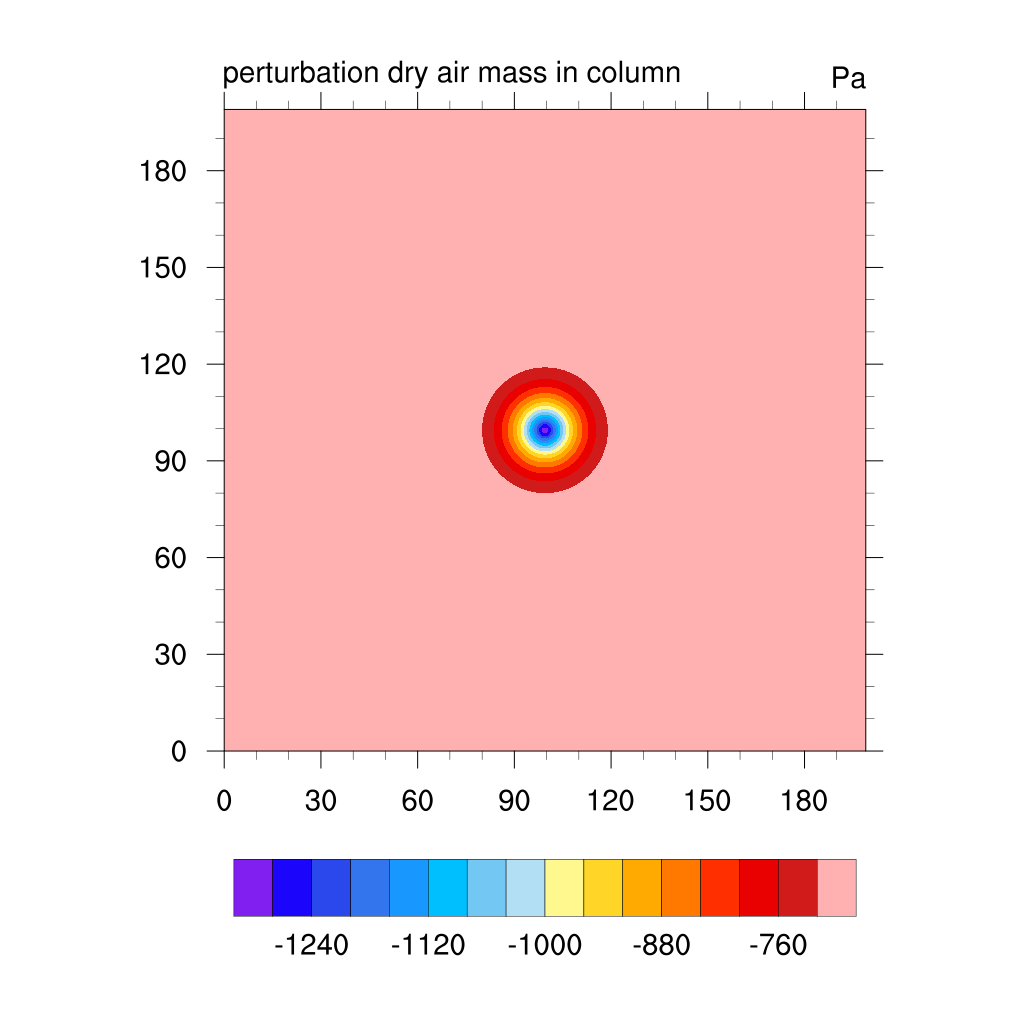
\includegraphics[height=10.25em]{images/coneff_000001.png}
					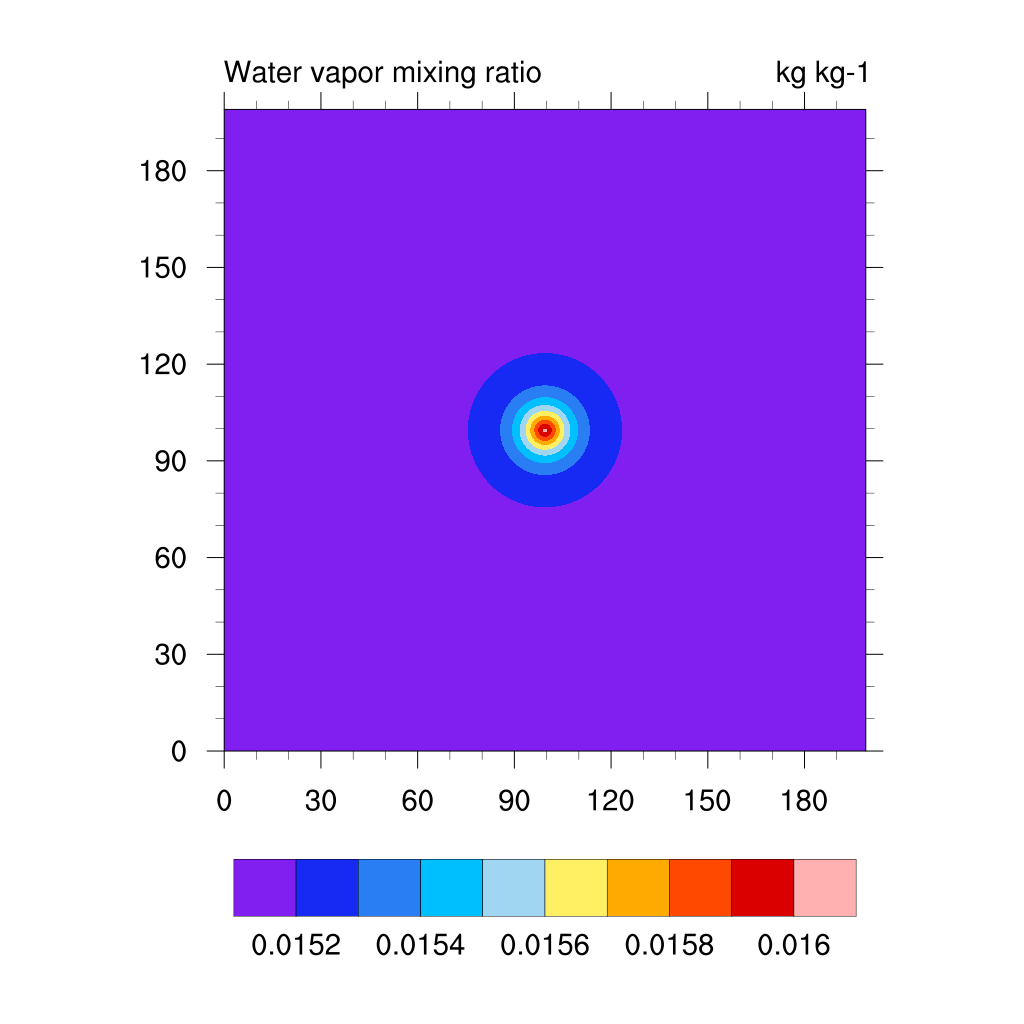
\includegraphics[height=10.25em]{images/coneff_000002.png}\\
					{\footnotesize \textbf{Figure 2.} Ideal case used for architecture verification: \textit{em\_tropical\_cyclone}, 30 days simulated.}
				\end{center}


			}




			%%%%%%%%%%%%%%%%%%%%%%%%%%%%%%%%%%%%%%%%%%%%%%%%%%%%%%%%%%%%%%%%%%%%%%%%%%%%%%
			\headerbox{{\textbf{\textcolor{white}{References}}}}{name=references,column=2,span=1,above=bottom}{
				%%%%%%%%%%%%%%%%%%%%%%%%%%%%%%%%%%%%%%%%%%%%%%%%%%%%%%%%%%%%%%%%%%%%%%%%%%%%%%
				\smaller
				\begin{multicols}{1}
					\bibliographystyle{ieee}
					\renewcommand{\section}[2]{\vskip 0.05em}
					\begin{thebibliography}{1}\itemsep=-0.01em
						\setlength{\baselineskip}{0.4em}

						\bibitem{dmontes2017}
						Montes, D.A. et al
						\newblock Enabling BOINC in infrastructure as a service cloud system
						\newblock \emph{Geosci. Model Dev., 10, 811-826, https://doi.org/10.5194/gmd-10-811-2017, 2017.}
						\bibitem{dmontes2018_egu}
						Montes, D.A. et al
						\newblock Insights on the use of WRF in Cloud Systems
						\newblock \emph{Geophysical Research Abstracts. Vol. 20, EGU2018-16881, 2018. EGU General Assembly 2018}
					\end{thebibliography}


				\end{multicols}
			}

			%%%%%%%%%%%%%%%%%%%%%%%%%%%%%%%%%%%%%%%%%%%%%%%%%%%%%%%%%%%%%%%%%%%%%%%%%%%%%%
			\headerbox{\textcolor{white}{\textbf{Acknowledgements}}}{name=acknowledge,column=3,span=1,above=bottom}{
				%%%%%%%%%%%%%%%%%%%%%%%%%%%%%%%%%%%%%%%%%%%%%%%%%%%%%%%%%%%%%%%%%%%%%%%%%%%%%%
				\smaller
        ~
				\begin{center}
					
\includegraphics[width=0.32\linewidth]{images/logo_google} \\
          ~
					This material is based upon work supported by \\ Google Cloud.
					~ \\~\\
				\end{center}
			}

			\end{poster}%
			%
\end{document}
